% This document describes the basement layout signaling system.
%
%  				J. Michael Dean, M.D.
%  				University of Utah School of Medicine

% The following line makes this document point back so that my software will synchronize
% between the preview and source windows.

%!TEX root = ../Railroad.tex

\chapter{Basement Layout Signaling System}
\minitoc

\section{Goals}

My layout is G-shaped with two staging yards attached (Figure \vref{fig:overallPlan});  the top of the layout is against the basement wall.  This means that conductors cannot simply follow their trains completely - there are areas where they will have to walk around to the other side of the layout to resume seeing their engine.  So I decided to place physical signals in locations that would warn conductors of ``what is around the corner''. Since I have three general areas, these need to have signals at each end, for a total of six signals.  Each area can be reached by the ground level primary main line as well as from an elevated ``mountain route'', so the total becomes 12 physical signals.

My primary goal is to have animation that demonstrates permissive ABS signaling.  Having detailed signals to mimic the prototype was NOT one of my goals - only a model railroad connoisseur would appreciate expensive detailed signal models.  The animation itself is entertaining for people to watch, and the signaling logic may pave the way for automated train dispatching in the future, using JMRI.  It is important to note that there are many more occupancy zones on the layout than 12, and this will have implications for the JMRI configuration later described in this document.

	\begin{landscape}
	\begin{figure}[htbp]
	\centering
	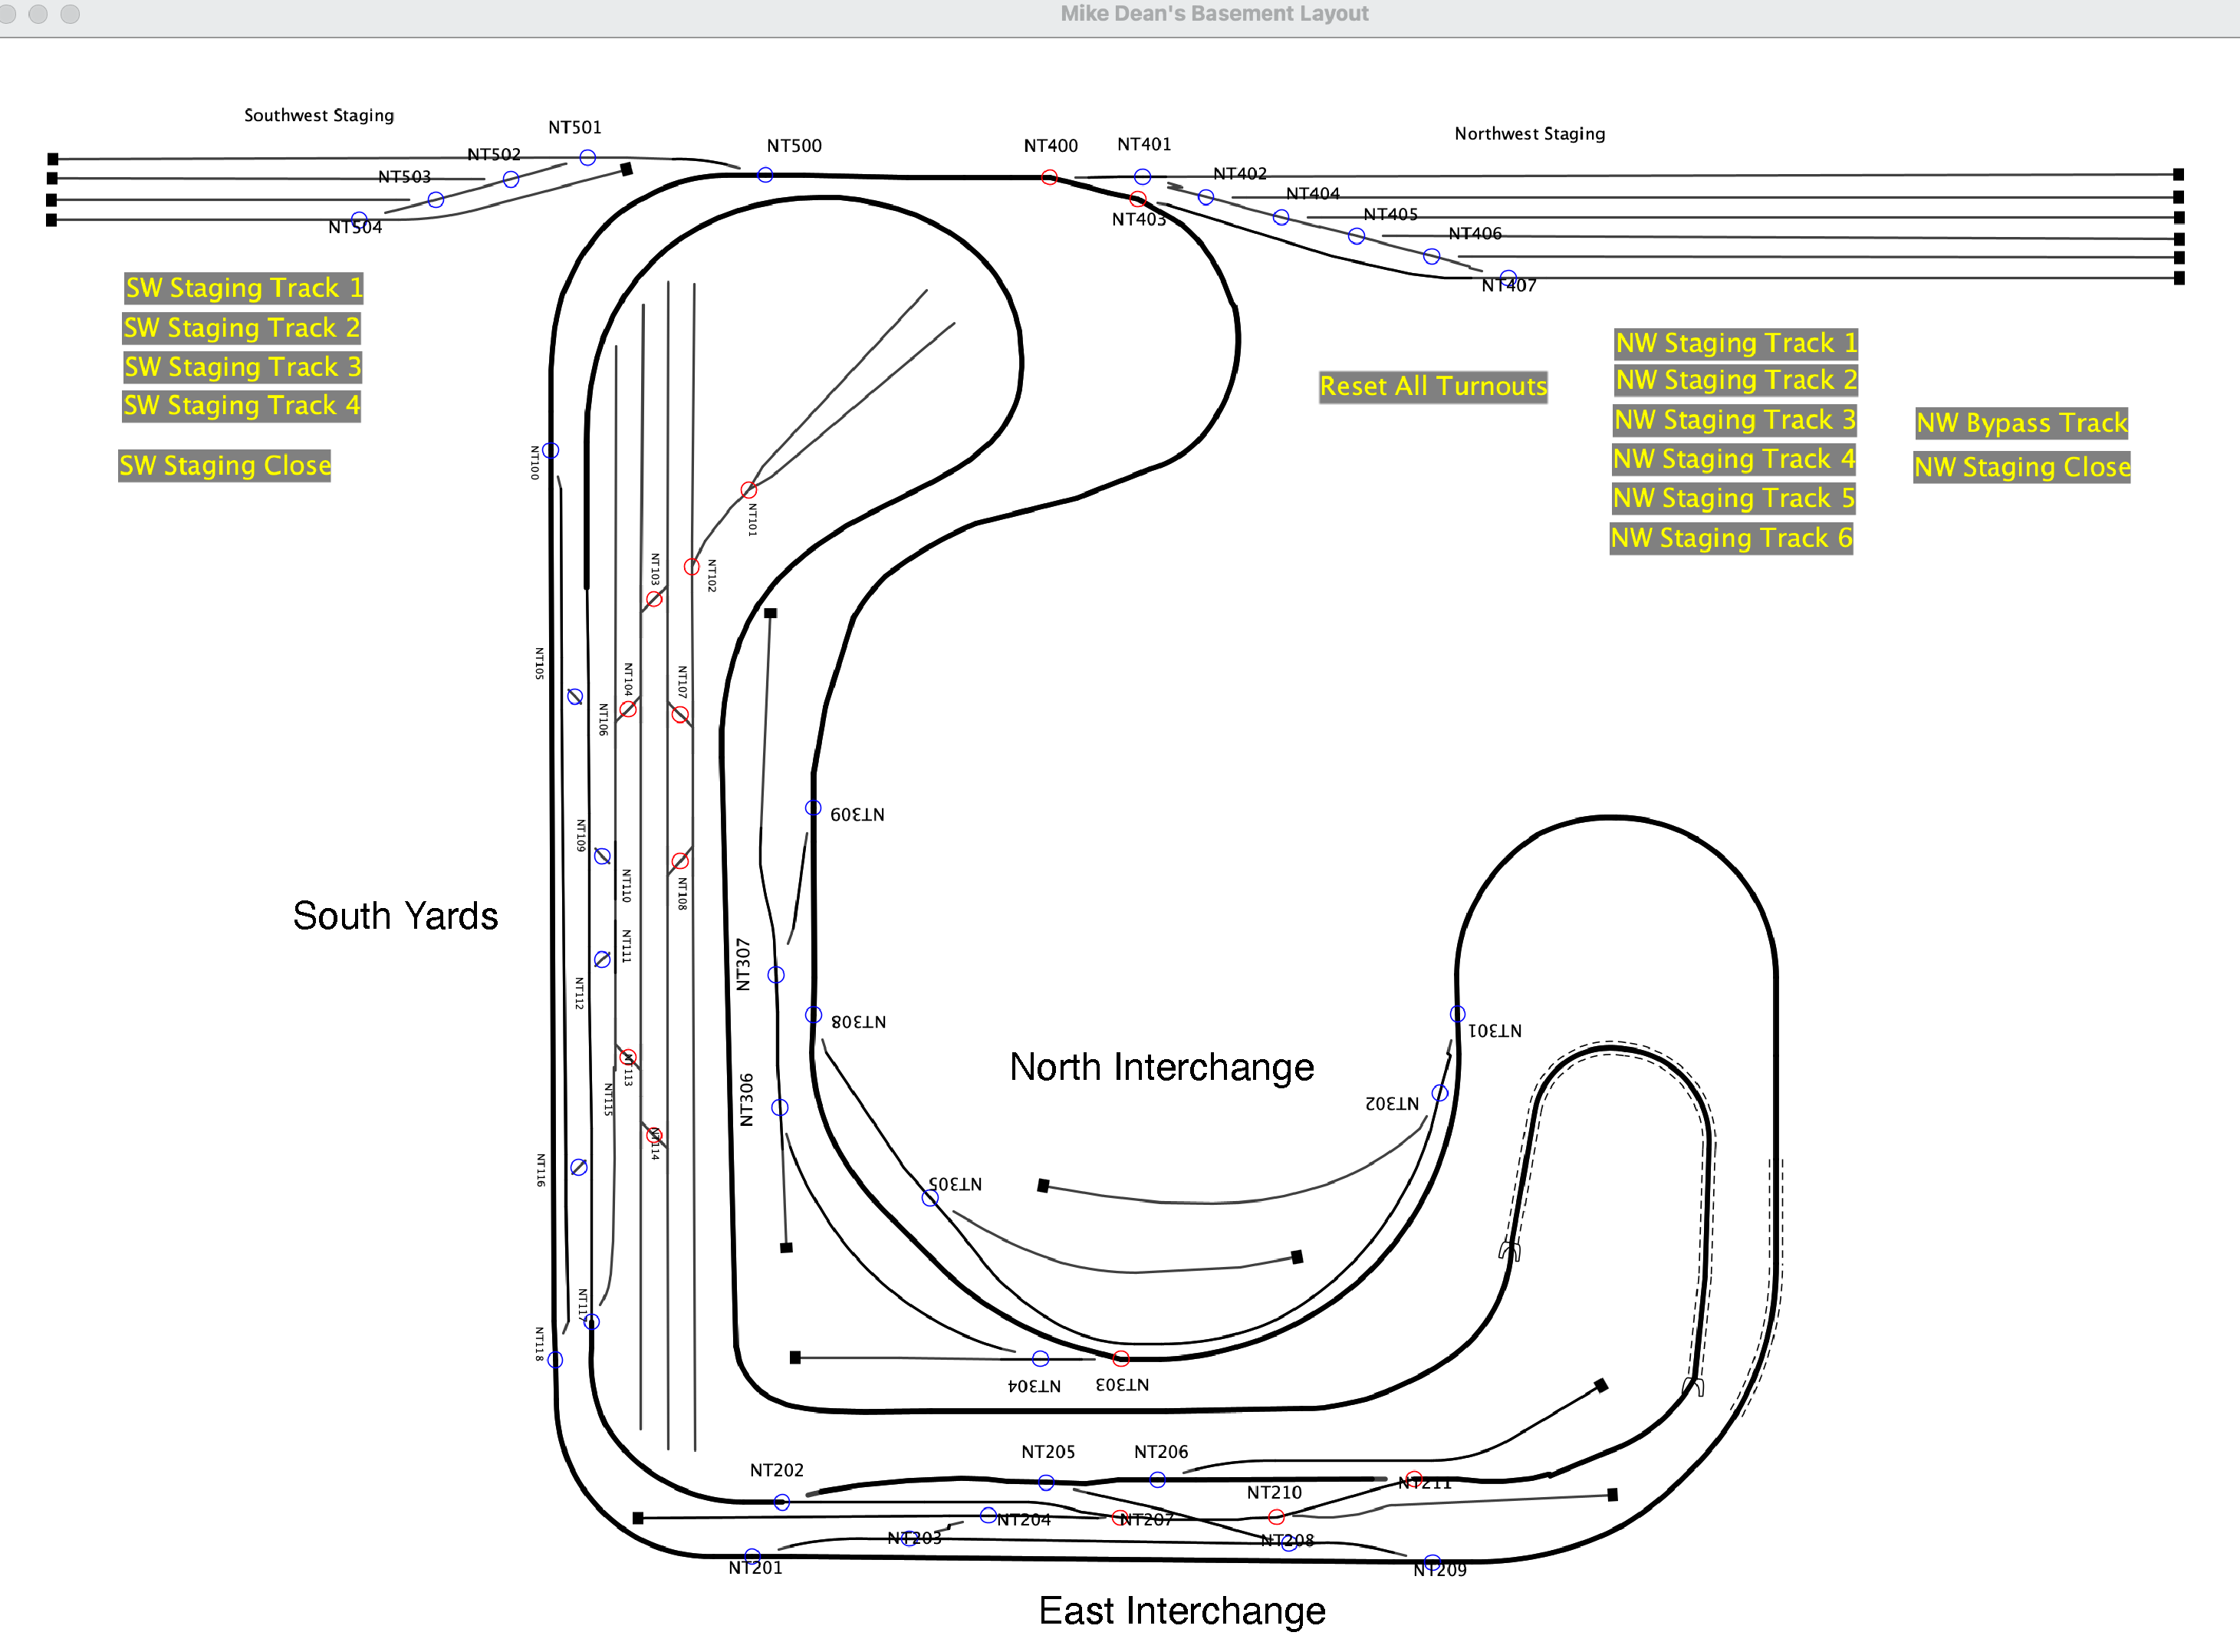
\includegraphics[width=\linewidth]{./electrical/figures/OverallPlan.pdf}
	\caption{Overall layout is shown here.  The staging areas are adjacent to the basement wall, preventing operators from walking completely around the layout to follow their trains.}
	\label{fig:overallPlan}
	\end{figure}
	\end{landscape}

\section{Underlying Layout Hardware}

Occupancy of blocks is monitored with current detectors.  I started with NCE BD20 detectors, which are single coil devices.  I purchased over 20 of these but eventually decided to replace them because I found them unreliable.  I currently have three different types of detectors.  Team Digital made BlocD8, which was a high density block detector with eight coils.  I purchased two of these;  the boards perform well but are no longer made (the company told me they did not sell enough to justify continued production).  I primarily replaced the BD20s with Model Railroad Control Systems cpOD, also a single coil device.  Finally, as I am a member of the Model Electronic Railway Group (MERG) based in the United Kingdom, I built several of their digital track circuit modules, DTC2 (Kit 50).  MERG distributes a large number of electronic modules as kits that must be assembled by the buyer.  They are very cost effective, but building two of these modules was sufficient to satisfy my appetite for soldering.

The occupancy detectors are connected to NCE AIU boards, which provides the detector signals to the NCE bus and ultimately to JMRI.  The AIU configuration is described in a separate document.

\section{JMRI Configuration}
